% TODO


\begin{figure}[htbp]
    \centering
    \makebox[\textwidth][c]{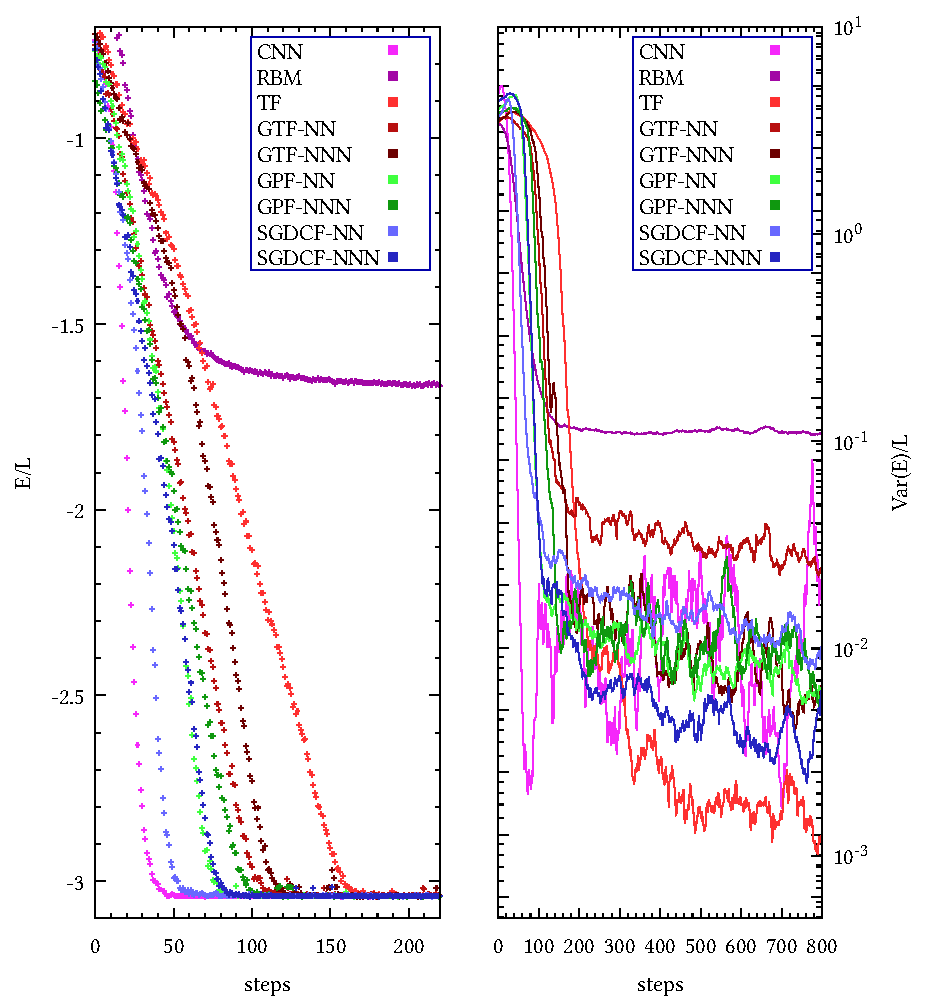
\includegraphics[width=1.1\textwidth]{./experiments/ground-state-search/comparison-established/architecture-comparison/architecture-comparison.pdf}}
    \caption{A comparison of different established and novel neural network architectures used as NQS in a ground state search.
        The calculations were performed for a 2D-trigonal\_hexagonal lattice of size 3 (37 lattice sites).
        The lattice is periodic and the encoding is set to be random.
        The models were configured to be as similar as possibly in terms of the number of trainable weights.
        The \emph{CNN} was set to have 16 channels ($\stackrel{\wedge}{=}$ 592 weights), The \emph{RBM} was set have 8 hidden layers ($\stackrel{\wedge}{=}$ 592 weights). 
        All metaformers were set to a depth of 2, and a mlp-ratio of 2.
        The poolformers have an embed-dimension of 7 ($\stackrel{\wedge}{=}$ 560 weights for \emph{GPF-NN} and 602 for \emph{GPF-NNN}).
        The conformers also have their embed dimension set to 7 ($\stackrel{\wedge}{=}$ 602 weights for \emph{SGDCF-NN} and 644 for \emph{SGDCF-NNN}).
        Finally the transformers are set to have an embed-dimension of 5 ($\stackrel{\wedge}{=}$ 530 weights for \emph{TF}, 566 weights for \emph{GTF-NN} and 596 weights for \emph{GTF-NN}). 
        Important to notice are the different scales of the x-axes. 
        The variance data is interpolated with a moving average in the logarithmic scale of width 35 steps.
    }
    \label{fig:gss-architectures-comp}
\end{figure}